\phantomsection
\section*{2. Topological Spaces}
\addcontentsline{toc}{section}{2. Topological Spaces}
\phantomsection
\subsection*{1. Topology}
\addcontentsline{toc}{subsection}{1. Topology}
\begin{customdefinition}{2.1}[Topology](Here's where everything starts to go south...)
\begin{enumerate}
    \item[1). ] Let $X$ be a set. A topology on $X$ is a set $\tau$ of subsets of $X$, called open sets, such that 
        \begin{enumerate}
            \item[i).] $\varnothing, \,\,X$ are open sets
            \item[ii).] If $\left\{U_i\right\}_{i \in I}$ is an arbitrary collection of open sets, then $\underaccent{i \in I}{\bigcup}U_i$ is open
            \item[iii).] If $\left\{U_i\right\}_{i \in I}$ is a finite collection of open sets, then $\underaccent{i \in I}{\bigcap}U_i$ is open
        \end{enumerate}
    \item[2). ]A topological space is a set $X$ with a chosen topology $\tau$.\\
            For example, the Euclidean topology on $\R^n$,  $\tau_{\text{Euclidean}} = \left\{U \subset \R^n \mid U \text{open in the sense of Definition 1.6}\right\}$
\end{enumerate}
\end{customdefinition}

\begin{customdefinition}{2.2}[Discrete Topology]
Let $X$ be a set. The discrete topology on $X$ is 
    $$\tau_{\text{dis}} = \left\{U \subset X\right\}$$
    That is, every subset of $X$ is open. It is immediate that $\tau_{\text{dis}}$ is indeed a topology.\\
Book: If $X$ is any set, the collection of all subsets of $X$ is a topology on $X$, it is called discrete topology.
\end{customdefinition}

\begin{customdefinition}{2.3}[Indiscrete(trivial) Topology]
Let $X$ be a set. The indiscrete(trivial) topology on $X$ is 
    $$\tau_{\text{ind}} = \left\{\varnothing, X\right\}$$
    That is, every subset of $X$ is open. It is immediate that $\tau_{\text{dis}}$ is indeed a topology.\\
The indiscrete topology is very ``small" in the sense that all points of $X$ are clumped together! On the other hand, the discrete topology is very ``large" (Spoiler Alert: is it Hausdorff?).\\
Book: The collection of consisting of $X$ and $\varnothing$ only is a topology on $X$, we shall call it the indiscrete topology.
\end{customdefinition}

\begin{customdefinition}{2.4}[The Finite Complement Topology]
Let $X$ be a set. The finite Complement topology on $X$ is 
    $$\tau_{\text{fin}} = \left\{U\subset X \mid X \setminus U \text{ is a finite set or is } X \right\}$$
    That is, every subset of $X$ is open. It is immediate that $\tau_{\text{dis}}$ is indeed a topology.\\
Book: Let $X$ be a set; let $\tau_f$ be the collection of all subsets $U$ of $X$ such that $X-U$ either is finite or is all of $X$. Then $\tau_f$ is a topology on $X$, called the finite complement topology. 
\end{customdefinition}
\begin{proof}
Check that $2.4$ is a topology
\begin{enumerate}
    \item[1).] $\varnothing \in \tau_f$ since $X\setminus X$ is finite. $X\in \tau_f$ since $X\setminus\varnothing$ is all of $X$.
    \item[2).] Say $\left\{U_i\right\}_{i\in I}$ are open, i.e.
               $$X \setminus U_i \text{ is finite on } X$$
               then
               $$X \setminus \underaccent{i \in I}{\bigcup}U_i = \underaccent{i \in I}{\bigcap}\left(X \setminus U_i\right)$$
               is the intersection of finite sets, so is itself finite. Hence, $\underaccent{i \in I}{\bigcup}U_i$ is open.
    \item[3).] Say $\left\{U_i\right\}_{i\in I}$ is a finite collection of open sets. Then
               $$X \setminus \underaccent{i \in I}{\bigcap}U_i = \underaccent{i \in I}{\bigcup}\left(X \setminus U_i\right)$$
               is a finite union of finite sets and so is itself finite. Hence, $\underaccent{i \in I}{\bigcap}U_i$ is open.          
\end{enumerate}
Therefore, $\tau_f$ is a topology.
\end{proof}

\begin{customdefinition}{2.5}[Coarser and Finer]
Let $X$ be a set with topologies $\tau$ and $\tau'$. We call $\tau$ coarser than $\tau \subset \tau'$. In this situation, we call $\tau'$ finer than $\tau$. If either $\tau \subset \tau'$ or $\tau' \subset \tau$, then we call $\tau$ and $\tau'$ comparable.
\end{customdefinition}

\newpage

\phantomsection
\subsection*{2. Basis for Topology}
\addcontentsline{toc}{subsection}{2. Basis for Topology}

\begin{customdefinition}{2.6}[Basis for a Topology]
Let $X$ be a set. A basis for a topology on $X$ is a collection $\B$ of subsets of $X$ such that
\begin{enumerate}
    \item[1).] Every $x \in X$ is contained in some $B \in \B$
    \item[2).] If $x\in X$ with $B_1, B_2 \in \B$ containing $x$ then there exists $B_3 \in \B$ such that 
                $$x\in B_3 \subset B_1 \cap B_2$$
                In pictures:
                \begin{center}
                \begin{tikzpicture}
                \draw[red, semitransparent, dashed, thick] (-1.5,0) circle[radius=66pt];
                \node[label, red] at (-1.6,1) {$B_1$};
                \draw[red, semitransparent, dashed, thick] (1.5,-1) circle[radius=88pt];
                \node[label, red] at (1.5,-1) {$B_2$};
                \draw[red, semitransparent, dashed, thick] (-0.3,-0.3) circle[radius=24pt];
                \node[label, blue] at (-0.3,-0.3) {$x$};
                \node[label, red] at (0,0) {$B_3$};
                \end{tikzpicture}
                \end{center}
    \end{enumerate} 
\end{customdefinition}


\begin{customthm}{2.1}
Let $\B$ be a basis for a topology on $X$. Then 
$$\tau = \left\{U \subset X \mid \text{ for all $u \in U$, there exists a $B \in \B$ such that $u \in B \subset U$}\right\}$$
is a topology on $X$.
\end{customthm}

\begin{customdefinition}{2.6}
The topology $\tau$ of Theorem $2.1$ is called the topology generated by $\B$.\\
Book: A subset $U$ of $X$ is said to be open in $X$ (that is, to be an element of $\tau$) if for each $x\in U$, there is a basis element $B \in \B$ such that $x \in B$ and $B \subset U$. Note that each basis element is itself an element of $\tau$.
\end{customdefinition}

\begin{customlemma}{2.2}
Let $\B$ be a basis for a topology $\tau$ on a set $X$. Then $U \subset X$ is open (i.e. $U\in \tau$) if and only if $U$ is a union of elements of $\B$.
\end{customlemma}

\begin{proof}
Given a collection of elements of $\B$, they are also elements in $\tau$. Because $\tau$ is a topology, their union is in $\tau$. Conversely, given $U \in \tau$, choose for each $x\in U$ an element $B_x$ of $\B$ such that $x \in B_x \subset U$. Then $U = \underaccent{x \in U}{\bigcup} B_x$, so $U$ equals a union of elements of $\B$. 
\end{proof}

\begin{customlemma}{2.3}
Let $(X, \tau)$ be a topological space. Let $\mathcal{C}$ be a collection of open sets such that for each open set $U$ and $x \in U$, there exists a $C\in \mathcal{C}$ such that $x \in C \subset U$. Then $\mathcal{C}$ is a basis for $\tau$.
\end{customlemma}

\begin{proof}
We need to show two things:
\begin{enumerate}
    \item[1).] $\mathcal{C}$ is a basis for a topology on $X$.\\
            The first condition for a basis is easy: Given $x\in X$, since $X$ is itself an open set, there is by hypothesis an element $C$ of $\mathcal{C}$ such that $x\in C \subset X$. To check the second condition, let $x$ belong $C_1 \cap C_2$, where $C_1$ and $C_2$ are elements of $\mathcal{C}$. Since $C_1$ and $C_2$ are open, so is $C_1 \cap C_2$. Therefore, there exists by hypothesis an element $C_3$ in $\mathcal{C}$ such that $x \in C_3 \subset C_1 \cap C_2$.
    \item[2).] The topology $\tau_{\mathcal{C}}$ generated by $\mathcal{C}$ is $\tau$.\\
            Let $U \subset X$ be open. For each $u \in U$, there exists a $C_u \in \mathcal{C}$ with $u \in C_u \subset U$. Then 
                    $$U = \underaccent{u \in U}{\bigcup} C_u$$
            By Lemma $2.2$, the right hand side is in $\tau_{\mathcal{C}}$, that is $\tau \subset \tau_{\mathcal{C}}$. Since $\mathcal{C} \subset \tau$, again by Lemma $2.2$, we have $\tau_{\mathcal{C}} \subset \tau$. So, $\tau = \tau_{\mathcal{C}}$.
\end{enumerate}
\end{proof}

\newpage

\begin{customdefinition}{2.7}
A subbasis $\mathcal{S}$ for a topology on $X$ is a collection of subsets of $X$ whose union is equal to $X$:
    $$\underaccent{S \in \mathcal{S}}{\bigcup}S = X$$
\end{customdefinition}

\begin{customlemma}{2.4}
Let $\mathcal{S}$ be a subbasis for a topology on $X$. Then 
$$\tau_{\mathcal{S}} = \left\{U \subset X \mid \text{ $U$ is a union of finite intersections of elements of $\mathcal{S}$}\right\}$$
is a topology on $X$.
\end{customlemma}

\phantomsection
\subsection*{3. Product Topology}
\addcontentsline{toc}{subsection}{3. Product Topology}

\begin{customdefinition}{2.8}[Product Topology]
Let $X, Y$ be topological spaces. The product topology on 
$$X \times Y = \left\{(x,y) \mid x\in X, y\in Y\right\}$$
is the topology generated by the basis 
$$\B = \left\{u \times v \mid u \subset X \text{ is open, } v\subset Y \text{ is open}\right\}$$
\end{customdefinition}

\begin{proof}
Check that $\B$ is indeed a basis for a topology on $X\times Y$.
\begin{enumerate}
    \item[1).] $\B$ covers $X \times Y$: Let $(x, y) \in X \times Y$. Since $X \subset X$ and $Y \subset Y$ are open, $X \times Y \in \B$ and $\B$ covers. Or, it's already trivial, since $X \times Y$ is itself a basis element.
    \item[2).] Say $u \times v, \,\, u' \times v' \in \B$ and 
                $$(x, y) \in (u\times v) \cap (u' \times v') = (u \cap u') \times (v \cap v')$$
                Since $u \cap u',\,\, v \cap v'$ are open, we have
                $$(u\times v) \cap (u' \times v') \in \B$$
\end{enumerate} 
\end{proof}

\begin{customthm}{2.5}
Let $X$ and $Y$ be topological spaces with bases $\B$ and $\mathcal{C}$, respectively, then 
    $$\mathcal{D} = \left\{u\times v\mid u\in \B, v \in \mathcal{C}\right\}$$
    is a basis for the product topology on $X \times Y$.
\end{customthm}

\begin{proof}
We will use Lemma $2.3$. So, let $W \subset X \times Y$ be open and $(x,y) \in W$. By the definition of the product topology,
$$W = \underaccent{i}{\bigcup} u_i \times v_i$$
for some $u_i \in \B$ and $v_i \in \mathcal{C}$. Then 
$$(x, y) \in \underbrace{u_j \times v_j}_{in \,\mathcal{D}} \subset W$$
for some $j$. By Lemma $2.3$, we are done.
\end{proof}

\begin{customdefinition}{2.9}[Projections]
Let $\pi_x: X \times Y \longrightarrow X$ be defined by the equation:
$$\pi_x(x,y) = x$$
Let $\pi_y: X \times Y \longrightarrow Y$ be defined by the equation:
$$\pi_y(x,y) = y$$
The maps $\pi_x$ and $\pi_y$ are called the projections of $X \times Y$ onto (surjective) its its first and second factors, respectively. Given any subset $U \subset X$ is open, we have
$$\pi_x^{-1}(U) = \left\{(x, y) \in X\times Y \mid x\in U\right\}$$
In particular, if $X$ and $Y$ are topological spaces and $U\subset X$ is open, then so too is $\pi_x^{-1}(U)$.
\end{customdefinition}

\begin{customthm}{2.6}
Let $X, Y$ be topological spaces. Then 
$$\mathcal{S} = \left\{\pi_x^{-1}(U) \mid U\subset X \text{ is open}\right\} \cup \left\{\pi_y^{-1}(U) \mid V\subset Y \text{ is open}\right\}$$
is a subbasis for the product topology on $X \times Y$.
\end{customthm}

\newpage

\begin{proof}
Let $\tau$ be the product topology on $X \times Y$ and $\tau_{\mathcal{S}}$ the topology generated by $\mathcal{S}$. It is immediate that $\tau_{\mathcal{S}} \subset \tau$. To see that $\tau \subset \tau_{\mathcal{S}}$, note that if $U \subset X$ and $V \subset Y$ are open, then 
$$\pi_x^{-1}(U) \cap \pi_y^{-1}(V) = U \times V \in \tau_{\mathcal{S}}$$
Since $\left\{U \times V \mid U \subset X \text{ open, } V \subset Y \text{ open}\right\}$ is a basis for $\tau$, we get $\tau \subset \tau_{\mathcal{S}}$.
\end{proof}

\phantomsection
\subsection*{4. Subspace Topology}
\addcontentsline{toc}{subsection}{4. Subspace Topology}

\begin{customdefinition}{2.10}[Subspace Topology]
Let $(X, \tau)$ be a topological space and $Y \subset X$ a subset. Then 
$$\tau_Y = \left\{Y \cap U \mid U \subset X \text{ is open}\right\}$$
is the subspace topology on $Y$. With this topology, $Y$ is called a subspace of $X$; its open sets consist of all intersections of opens sets of $X$ and $Y$.
\end{customdefinition}

\begin{customlemma}{2.7}
The subspace topology $\tau_Y$ is a topology.
\end{customlemma}
\begin{proof}
We have
\begin{align*}
    \varnothing &= Y \cap \varnothing \in \tau_Y\\
    Y & = Y \cap X \in \tau_Y
\end{align*}
Let $\left\{U_i\right\}_{i \in I}$ be open in $Y$ (so $U_i \in \tau_Y$). Then 
$$U_i = Y\cap V_i$$
for some $V_i \subset X$ open and 
\begin{align*}
  \underaccent{i\in I}{\bigcup} U_i &= Y \cap \underbrace{\left(\underaccent{i\in I}{\bigcup} V_i\right)}_{\text{open in $X$}} \in \tau_Y \\
  \underaccent{i\in I}{\bigcap} U_i &= Y \cap \overbrace{\left(\underaccent{i\in I}{\bigcap} V_i\right)}_{} \in \tau_Y
\end{align*}
if $|I| < \infty$.
\end{proof}

\begin{customlemma}{2.8}
Let $Y \subset X$ be a subspace. If $U \subset Y$ is open and $Y \subset U$ is open, then $U \subset X$ is open.
\end{customlemma}

\begin{proof}
Since $U$ is open in $Y$, $U = Y \cap V$ for some set $V$ open in $X$. Since $Y$ and $V$ are both open in $X$, so is $Y \cap V$.
\end{proof}

\begin{customlemma}{2.9}
Let $X$ be a topological space with basis $\B$ and $Y\subset X$ a subset. Then
$$\B_Y = \left\{Y\cap B \mid B \in \B\right\}$$
is a basis for the subspace topology of $Y$. In words, a basis for $X$ induces a basis for the subspace $Y \subset X$.
\end{customlemma}

\begin{proof}
Given $U$ is open in $X$ and given $y \in U \cap Y$, we can choose an element $B$ of $\B$ such that $y \in B \subset U$. Then $y \in B \cap Y \subset U \cap Y$. It follows from Lemma $2.3$ that $\B_Y$ is a basis for the subspace topology on $Y$.
\end{proof}

\begin{customthm}{2.10}
Let $X, Y$ be topological spaces with subsets $A\subset X$ and $B \subset Y$. Then the subspace topology on $A\times B \subset X \times Y$ is the same as the product topology on $A \times B$.
\end{customthm}

\begin{proof}
A basis element of the product topology on $X \times Y$ is $U\times V$, where $U\subset X$ and $V \subset Y$ are open. Then 
$$\left(A \times B\right) \cap \left(U \times V\right) = \left(A\cap U\right) \times \left(B \cap V\right)$$
is a basis element for the subspace topology on $A \times B$. But the RHS is a basis element for the product topology on $A\times B$.
\end{proof}

\begin{customdefinition}{2.11}
Let $X$ be a topological space. A subset $A \subset X$ is called closed if $A^c = X \setminus A \subset X$ is open.
\end{customdefinition}

\begin{customthm}{2.11}
Let $X$ be a topological space
\begin{enumerate}
    \item[1).] $\varnothing$ and $X$ are closed.
    \item[2).] Arbitrary intersections of closed sets are closed:\\
                If $\left\{A_i\right\}_{i \in I}$ is a collection of closed sets, then $\underaccent{i\in I}{\bigcap} A_i$ is closed.
    \item[3).] Finite unions of closed sets are closed:\\
                If $\left\{A_i\right\}_{i \in I}$ is a finite collection of closed sets, then $\underaccent{i\in I}{\bigcup} A_i$ is closed.
\end{enumerate}
\end{customthm}

\newpage

\begin{proof}
\begin{enumerate}
    \item[1).] $\varnothing$ and $X$ are closed because they are the complements of the open sets $X$ and $\varnothing$, respectively.
    \item[2).] Given a collection of closed sets $\left\{A_i\right\}_{i \in I}$, we apply DeMorgan's Law,
        $$X - \underaccent{i \in I}{\bigcap} A_i = \underaccent{i\in I}{\bigcup} \left(X - A_i\right)$$
        Since the sets $X - A_i$ are open by definition, the right side of this equation represents an arbitrary union of open sets, and is thus open. Therefore, $\underaccent{i \in I}{\bigcap} A_i$ is closed.
    \item[3).] Similarly, if $A_i$ is closed for $i = 1, 2, \dots, n \in I $, consider the equation
        $$X - \underaccent{i \in I}{\bigcup} A_i = \underaccent{i\in I}{\bigcap} \left(X - A_i\right)$$
        The set on the right hand side is a finite intersection of open sets and is therefore open. Hence $\underaccent{i \in I}{\bigcup} A_i$ is closed.
\end{enumerate}
\end{proof}

\begin{customlemma}{2.12}
Let $Y \subset X$ be a subspace and $A \subset Y$ a subset. Then $A\subset Y$ is closed if and only if $A = Y \cap C$ for a closed set $C \subset X$. 
\end{customlemma}

\begin{proof} If and only if...
\begin{enumerate}
    \item[1).]Assume $A\subset Y$ is closed. Then $Y \setminus A$ is open so that $Y \setminus A = Y \cap U$ for an open $U \subset X$. Then
    \begin{align*}
        A & = Y \setminus\left(Y\setminus A\right)\\
          & = Y \setminus\left(Y \cap U\right)\\
          & = Y \cap \left(X \setminus U\right)
    \end{align*}
    The set $X \setminus U$ is closed in $X$, so we can take $C = X \setminus U$.
    \item[2).]Conversely, assume that $A = Y\cap C$ for $C \subset X$ closed. Then, by the above, we see that
    $$Y \setminus A = Y \cap \left(X \setminus C\right)$$
    The set $X \setminus C$ is open in $X$, so that $Y \setminus A$ is open in $Y$. Therefore, $A \subset Y$ is closed.
\end{enumerate}
\end{proof}

\phantomsection
\subsection*{5. Interior and Closure}
\addcontentsline{toc}{subsection}{5. Interior and Closure}

\begin{customdefinition}{2.12}[Interior and Closure]
Let $X$ be a topological space and $Y \subset X$ a subset.
\begin{enumerate}
    \item[1).] The interior of $Y (\text{in }X)$ is the union of all open sets contained in $Y$, and is denoted by $Int(Y)$.
    \item[2).] The closure of $Y (\text{in }X)$ is the intersection of all closed sets of $X$ which contain $Y$, and is denoted by $\overline{Y}$.
\end{enumerate}
$$Int(Y) \subset Y \subset \overline{Y}$$
If $Y$ is open, $Y = Int(Y)$; while if $Y$ is closed, $Y = \overline{Y}$
\end{customdefinition}

\begin{customlemma}{2.13}
Let $X$ be a topological space and $Y \subset X$ a subset. Then $Int(Y) \subset X$ is open and $\overline{Y} \subset X$ is closed.
\end{customlemma}

\begin{customlemma}{2.14}
Let $X$ be a topological space and $Y \subset X$ a subset.
\begin{enumerate}
    \item[1).] $Y$ is open if and only if $Int(Y) = Y$
    \item[2).] $Y$ is closed if and only if $Y = \overline{Y}$
\end{enumerate}
\end{customlemma}

\begin{customthm}{2.15}
Let $X$ be a topological space with a subset $Y$.
\begin{enumerate}
    \item[1).] Then $x \in \overline{Y}$ if and only if any open set $x\in U \subset X$ intersects $Y$.
    \item[2).] Let $\B$ be a basis for the topology on $X$. Then $x \in \overline{Y}$ if and only if every $B \in \B$ with $x \in B$ intersects $Y$.
\end{enumerate}
\end{customthm}

\begin{customdefinition}{2.13}[Limit Points]
Let $X$ be a topological space and $Y \subset X$ a subset. A point $l \in X$ is called a limit point of $Y$ (or cluster/accumulation point) if every open set $U \subset X$ which contains $l$ intersects $Y$ at a point different from $l$. Said differently, $l$ is a limit point of $A$ if it belongs to the closure of $A - \left\{x\right\}$. The point $l$ may lie in $A$ or not; for this definition it does not matter.
\end{customdefinition}

\begin{customthm}{2.16}
Let $X$ be a topological space with a subset $Y \subset X$. Then
$$\overline{Y} = Y \cup \left\{\text{limit points of Y}\right\} = Y \cup Y'. \,\,\,\,\,\,\, (Y' := \left\{\text{limit points of Y}\right\})$$
\end{customthm}

\begin{proof}
Let $l$ be a limit point of $Y$. Then every open set containing $l$ intersects $Y$. By Theorem $2.15$, $x\in \overline{Y}$. Hence, $\overline{Y} \supset Y \cup Y'$. For the reverse inclusion, let $x \in \overline{Y}$. Say $x \notin Y$; we prove that $x\in Y'$. Again by Theorem $2.15$, any open set $x \in U \subset X$ intersects $Y$. Since $x\notin Y$, we see that any open set containing $x$ intersects $Y$ at a point different from $l$. So, $x \in Y'$.
\end{proof}

\begin{customcoro}{2.17}
A subset $Y \subset X$ is closed if and only if it contains all of its limit points.
\end{customcoro}

\begin{customdefinition}{2.13}[Boundary]
Let $X$ be a topological space. The \emph{boundary} of a subset $A \subset X$ is defined to be
$$\partial A = \overline{A} \cap \overline{X \setminus A},$$
where $\overline{(-)}$ denotes closure.
\end{customdefinition}

\phantomsection
\subsection*{6. Hausdorff Spaces}
\addcontentsline{toc}{subsection}{6. Hausdorff Spaces}

\begin{customdefinition}{2.14}[Hausdorff Spaces]
A topological space $X$ is called Hausdorff if for every pair of distinct points $x, x' \in X$, there exists open sets 
$$x \in U \subset X,\,\,\,\,\,\,\, x' \in U' \subset X$$
such that $U \cap U' = \varnothing$\\
In pictures:
    \begin{center}
    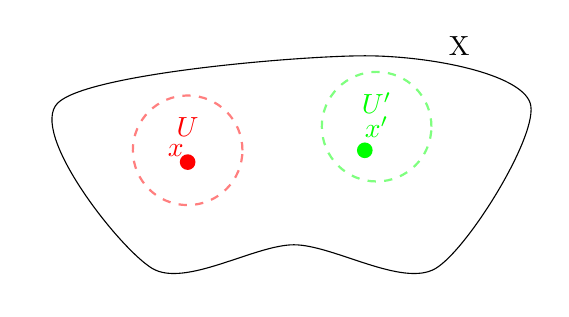
\begin{tikzpicture}[scale = 0.3]
    \draw[red, semitransparent, dashed, thick] (-4.5,-2) circle[radius=66pt];
    \node[label, red] at (-4.5,-1) {$U$};
    \node[label, red] at (-5,-2) {$x$};
    \node[circle, fill, red, inner sep=2pt] at (-4.5, -2.5) {};
    \draw[green, semitransparent, dashed, thick] (3.5,-1) circle[radius=66pt];
    \node[label, green] at (3.5,0) {$U'$};
    \node[label, green] at (3.5,-1) {$x'$};
    \node[circle, fill, green, inner sep=2pt] at (3, -2) {};
    \draw plot [smooth cycle] coordinates {(0,-6) (-6,-7) (-10,0) (3,2) (10,0) (6,-7) } node at (7,2.4) {X};
    \end{tikzpicture}
    \end{center}
\end{customdefinition}

\begin{customthm}{2.18}
Let $X$ be a Hausdorff (topological) space. Then any finite subset $A \subset X$ is closed. In particular, points are closed in $X$. 
\end{customthm}

\begin{customdefinition}{2.15}
Let $X$ be a topological space. A sequences of points $\left\{x_n\right\}_{n \geqslant 1}$ in $X$ converges to $x \in X$ if for any open set $x \in U \subset X$, there exists an $N > 0$ such that $x_n \in U$ whenever $n>N$.
\end{customdefinition}

\begin{customthm}{2.19}
Let $X$ be a Hausdorff space. A sequence in $\left\{x_n\right\}_{n \geqslant 1}$ in $X$ converges to at most one point of $X$; if it exists, this point is called the limit of $\left\{x_n\right\}$ and denoted by $\displaystyle\lim_{n \to \infty} x_n$.
\end{customthm}

\begin{proof}
Suppose that $\left\{x_n\right\}_{n \geqslant 1}$ converges to distinct points $a, b \in X$. Since $X$ is Hausdorff, there exists open set 
$$a \in U \subset X, \,\,\,\, b \in V \subset X$$
such that $U \cap V = \varnothing$. Since $\left\{x_n\right\}_{n \geqslant 1}$ converges to $a$, there exists $N > 0$ such that $x_n \in U$ if $n>N$. Similarly, there exists an $M>0$ such that $x_n \in V$ if $n>M$. Let $L = max\left\{M,N\right\}$. Then $x_n \in U\cap V$ if $n > L$. But $U\cap V = \varnothing$, a contradiction.
\end{proof}

\begin{customthm}{2.20}[Fantastic Top-spaces and Where to Find Them](Hausdorff)
\begin{enumerate}
    \item[1).] Let $X, Y$ be Hausdorff spaces. Then $X \times Y$ is Hausdorff.
    \item[2).] Let $X$ be a Hausdorff space and $Y \subset X$ a subset. Then $Y$, with the subspace topology, is Hausdorff.
\end{enumerate}
\end{customthm}

\begin{proof}
\begin{enumerate}
    \item[1).]Let $(x, y), (x', y') \in X\times Y$ be distinct. Suppose that $x \neq x'$. Since $X$ is Hausdorff, there exist open sets 
    $$x \in U \subset X, \,\,\,\,\,\, x' \in U' \subset X$$
    such that $U\cap U' = \varnothing$. Then 
    $$(x, y) \in U \times Y, \,\,\,\,\,\, (x', y') \in U' \times Y$$
    are disjoint open sets. If $x = x'$, then $y = y'$ and we can modify the previous argument.
    \item[2).]Let $y, y'\in Y$ be distinct. Since $X$ is Hausdorff, there exist open sets $y \in U \subset X, \,\, y' \in U' \subset X$ such that $U\cap U' = \varnothing$. Then $y \in U \cap Y \subset Y,\,\, y' \in U' \cap Y \subset Y$ are open sets in $Y$ such that 
    $$\left(U \cap Y \right) \cap \left(U' \cap Y \right) = \left(U \cap U' \right)\cap Y = \varnothing$$
    So, $Y$ is Hausdorff.
\end{enumerate}
\end{proof}